\documentclass{report}

% Packages
\usepackage[utf8]{inputenc}
\usepackage{graphicx}
\usepackage{enumitem}
\usepackage[siunitx, european]{circuitikz}
\usepackage{hyperref}
\usepackage{gensymb}
\usepackage{listings}

% Setup
\graphicspath{{img/}}
\title{Report Wetterstation mit einem Einplatinenrechner}
\author{Oliver Siegemund}
\date{Dezember 2023}
\setenumerate[0]{label=(\roman*)}
\setenumerate[1]{label=(\alph*)}


\begin{document}
\maketitle
Dokumentation der Entwicklung und Auswertung einer Wetterstation basierend auf dem daisy seed Einplatinenrechnern und alanogen Sensoren.
\pagebreak
\tableofcontents
\pagebreak
\chapter{Einleitung}
\section{Aufgabenstellung}
Du möchtest eine eigene Wetterstation bauen. Hierzu nutzt du einen Einplatinenrechner (z.B. Arduino) sowie zugehörige Sensoren.
\begin{enumerate}
	\item Lege eine Schaltung zur Erfassung der beiden Messgrößen Temperatur und Luftfeuchtigkeit aus und setze diese als Hardware um.
	\item Nehme mindestens 5 Messreihen bei unterschiedlichen Temperaturen und Luftfeuchtigkeitswerten auf (z.B. in verschiedenen Räumen oder Außenbereichen). Für jede Messreihe nehme dabei mindestens jeweils 100 Werte der beiden Messgrößen als Wiederholmessung auf.
	\item Beschreibe allgemein die Quantisierungsabweichung der Datensätze, die mithilfe des Einplatinenrechners aufgenommen wurden und stelle diese als Funktion der Bit-Zahl dar. Ermittle diese Abweichung für deinen konkreten Anwendungsfall.
	\item Ermittle die Messunsicherheit der Ausgangsgrößen Temperatur und Luftfeuchtigkeit auf drei verschiedene Arten – gebe als Ergebnis jeweils ein 95% Vertrauensintervall an:
\begin{enumerate}
	\item Auf Basis der statistischen Analyse Ihrer Messreihen aus Teil b).
\item Auf Basis der Informationen der Datenblätter der beiden Sensoren (a priori Wissen). Nutze die im Datenblatt vorhandene Information, um eine Bilanz der Messunsicherheit unter Nutzung des Guide to the Expression of Uncertainty in Measurement (GUM) sowie der hierin vorgesehenen Abweichungsfortpflanzung abzuleiten.
\item Über eine Messung der Spannung. Nutze deinen Einplatinenrechner um Messreihen der Spannung des Sensors sowie der zugehörigen Temperatur und Luftfeuchtigkeit aufzunehmen. Stelle auf Basis der in c) ermittelten Quantisierungsabweichung und anderer Einflüsse der Unsicherheit der Spannungsmessung eine Bilanz der Unsicherheit unter Nutzung des Guide to the Expression of Uncertainty in Measurement (GUM) sowie der hierin vorgesehenen Abweichungsfortpflanzung für die Ausgangsgrößen Temperatur und Luftfeuchtigkeit auf. Stelle dabei das mathematische Modell der Messung als Taylor-Reihe zweiter Ordnung dar. Interpretiere und vergleiche das Ergebnis auf Basis der drei Methoden. Diskutiere die jeweiligen Vorteile und Nachteile der drei Methoden auf Basis der Ergebnisse.
\end{enumerate}
Hinweise: Die Messung der Spannung kann entweder zeitgleich mit der Aufnahme der Ergebnisse von Temperatur und Spannung in Teil b) durchgeführt werden oder durch eine separate Messreihe.
Die Unsicherheitsbilanzierung und Systemmodellierung müssen durch Implementierung als Programm-Code
erfolgen.
Die Aufgabenteile i)-iii) können unabhängig voneinander gelöst werden.
\item Modelliere den Wärmeübergang auf den Temperatur-Sensor aus der Umgebungsluft mithilfe einer
Differentialgleichung 1. Ordnung und stelle das zeitliche Verhalten des Sensorsystems auf Basis der
Sprungantwort und Impulsantwort eines PT1-Systems für jeweils ein selbst gewähltes Szenario dar. Diskutiere,
welche Konsequenzen sich für die Wetterstation ergeben.
Hinweise zur Thermodynamik: Der Widerstand kann als perfekter Zylinder angenommen werden. Von
Interesse ist die Temperatur in seinem Kern. Der Wärmestrom \begin{math} q\left(t\right)\end{math} ist nach dem Fourier’schen Gesetz definiertc als:
\begin{displaymath}
q\left(t\right) = \lambda \frac{A}{r} \left(\vartheta_u\left(t\right) - \vartheta_r\left(t\right) \right)
\end{displaymath}
Hierbei bezeichnen $\vartheta_u\left(t\right)$ die Umgebungstemperatur, $\vartheta_r\left(t\right)$ die Kerntemperatur des Widerstands, $A$ seine Außenfläche, $r$ seinen Radius und $\lambda$ die materialabhängige Wärmeleitfähigkeit. 

Die Temperatur des Widerstands sowie der Wärmestrom hängen wie folgt zusammen:
\[
\frac{1}{c_{p,R}}\int{q\left(t\right) dt} = \vartheta_r\left(t\right)
\]
$c_{p,R}$ ist die spezifische Wärmekapazität und hängt vom Material des Widerstands ab. 

Die beiden Gleichungen können zu einer DGL 1. Ordnung für $\vartheta_r\left(t\right)$ kombiniert werden.

\end{enumerate}
\section{Hardware}
\subsection{Einplatinenrechner}
\begin{figure} [h!]
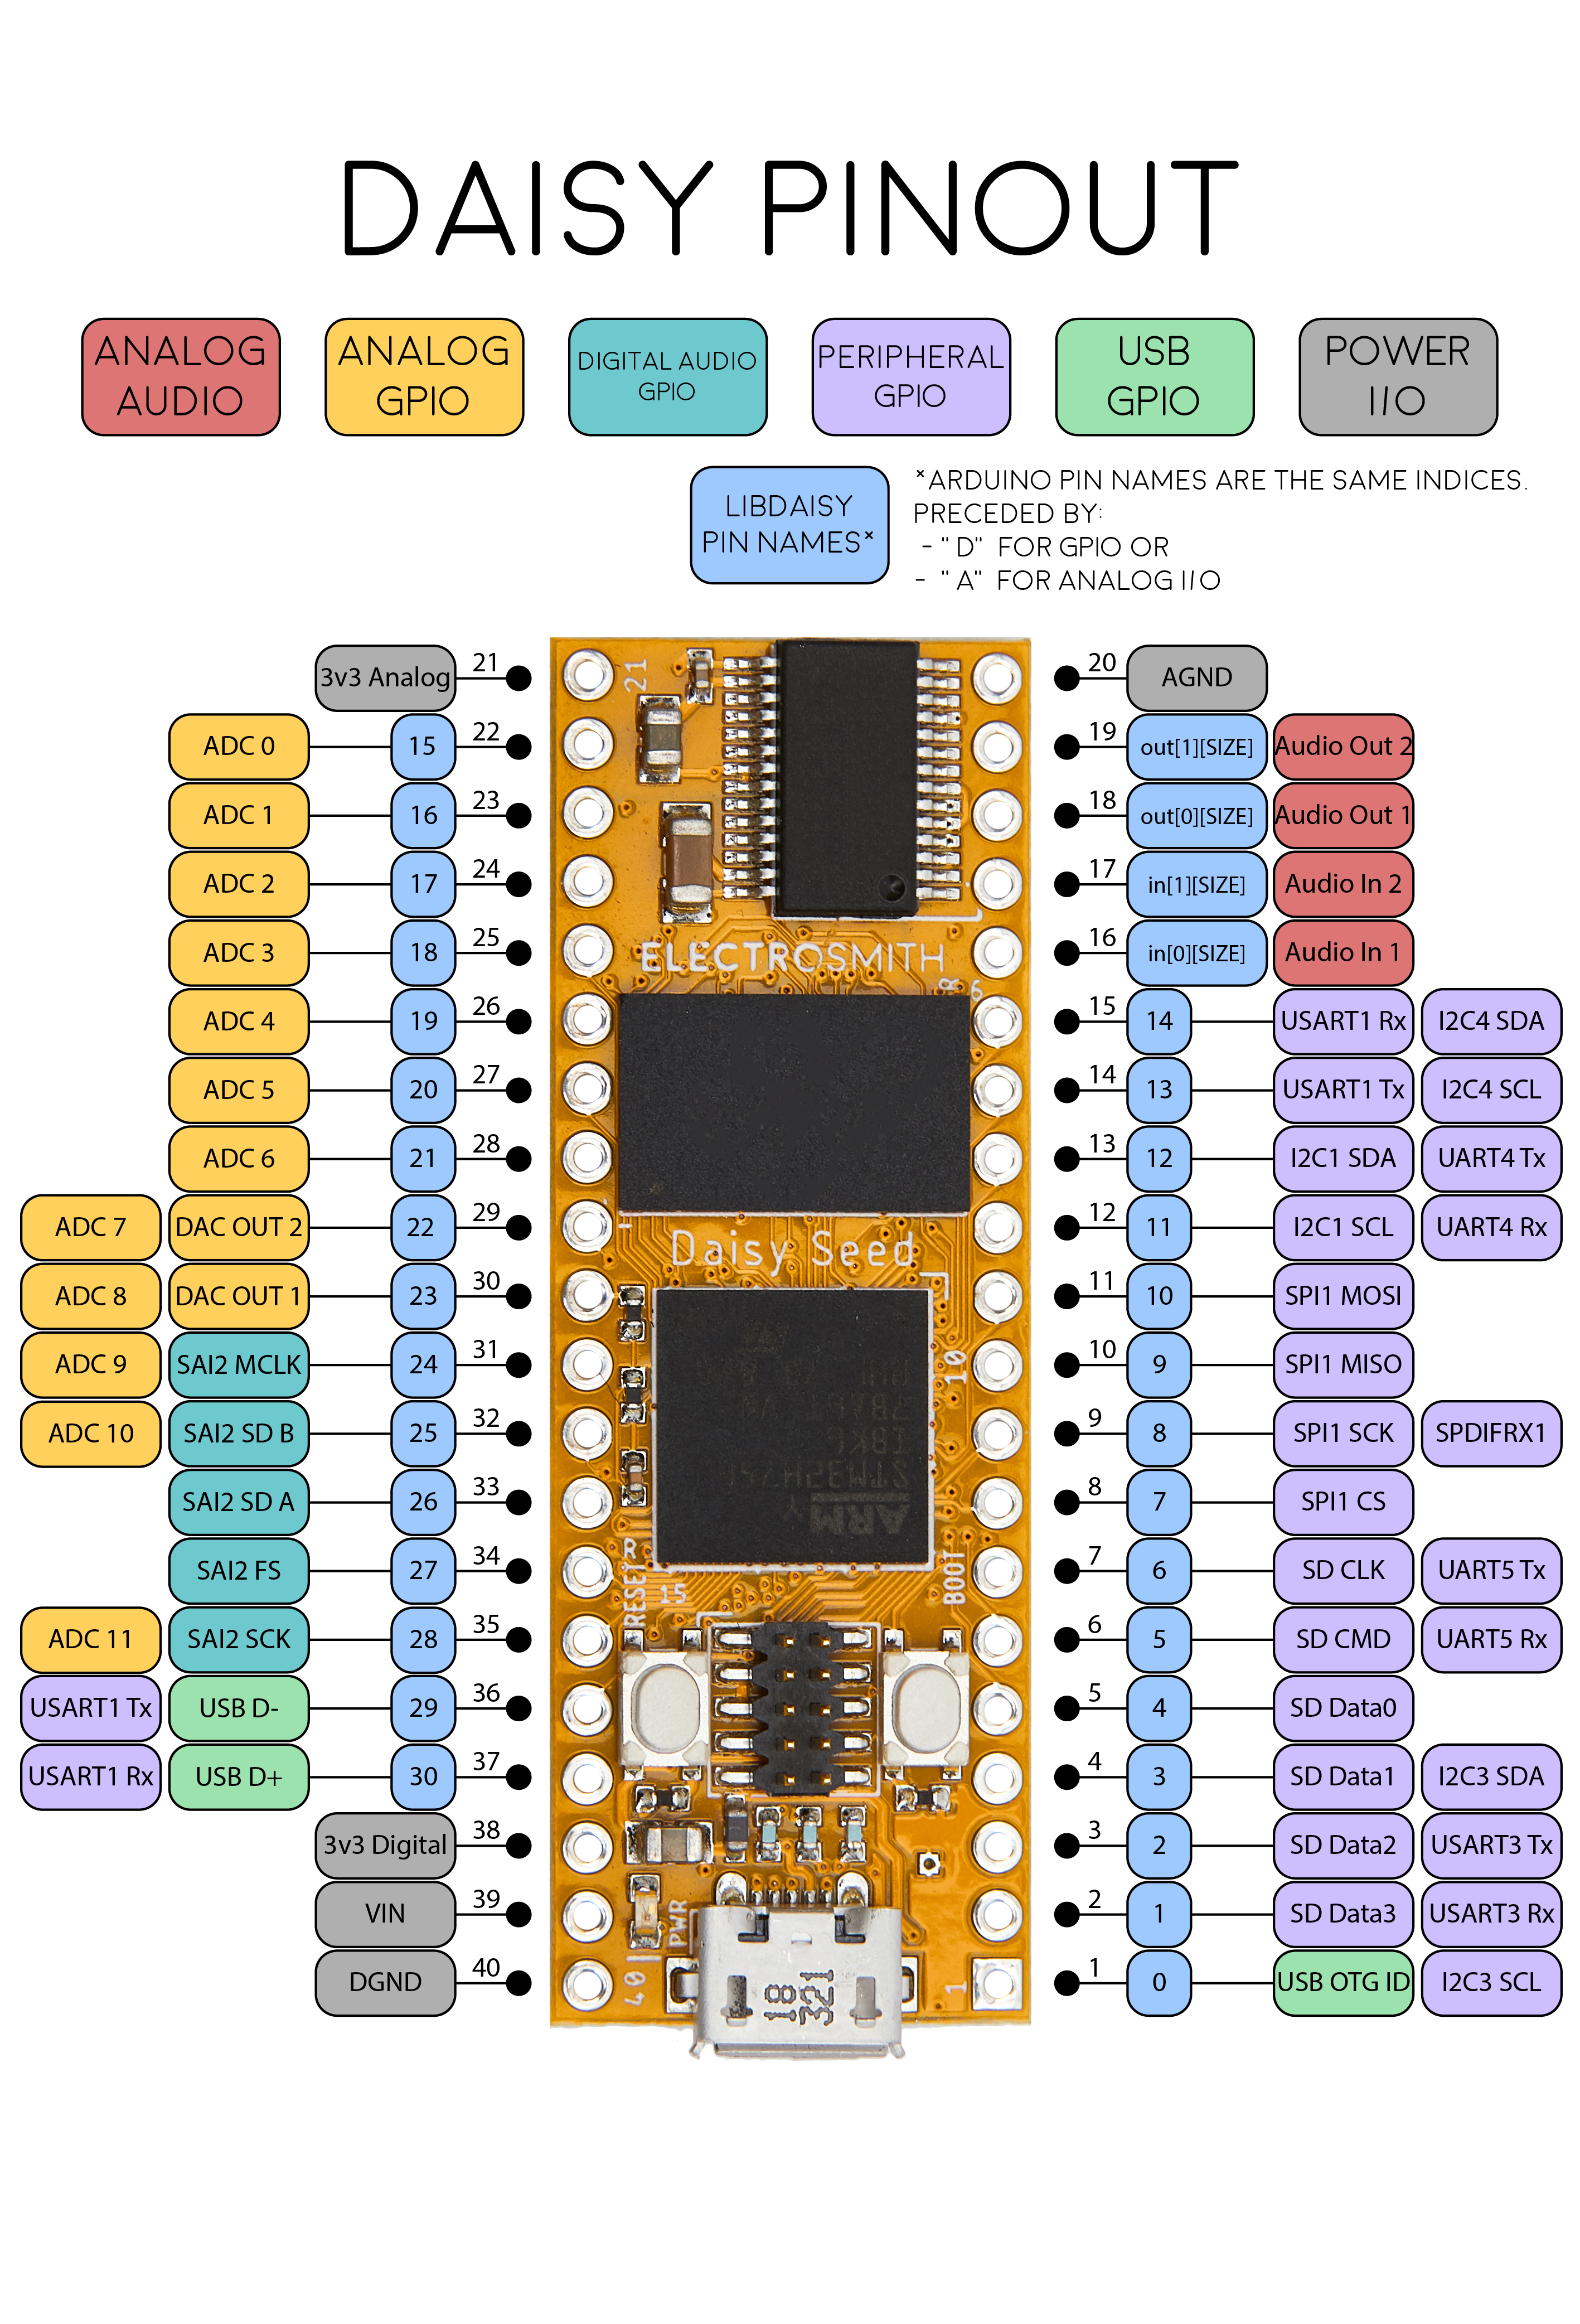
\includegraphics[width=0.75\textwidth]{daisy_seed_pinout}
\caption{daisy seed - Pinout}
\label{fig:daisy-ssed-pinout}
\end{figure}
\begin{center}

Fuer die Aufgabenstellung wurde der daisy seed rev7 gewaehlt. Neben der Tatsache das das Board verfuegbar ist, hat es sowie der verbaute STM32H750IB sehr gute Eigenschaften \cite{stm32h750} um Analoge Signale zu erfassen.

\begin{tabular} {| p{12em} | p{20em} |}
\hline
\multicolumn{2}{|c|}{Eigenschaften} \\
\hline
Analog Digital Konverter & 3 Wandler Kanaele mit bis zu 18bit Aufloesung auf 11 Pins \\
\hline
Digital Analog Konverter & 2 12-bit Digital / Analog Wandler mit bis zu 1 MHz \\
\hline
FPU & FPU mit doppelter Praezision \\
\hline
RAM & 64 MB SDRAM um Messwerte zu speichern ($\approx$ 2 Mega-Samples )\\
\hline
\end{tabular}
\end{center}

\subsection{Sensoren}
\subsubsection{Temperatur}
Zur Termperaturmessung wurde ein Termistor gewahlet. Genauer der KTY 81 122m mit einem Temperatur Koeffizenten $T_C$ von 0.79 und einem Widerstand bei $T_a = 25 \degree C$ zwischem 1000 und 1020 $\Omega$ ausweist, laut Hersteller Datenblatt. Ausgelegt ist der Sensor fuer einen Temperaturbereich zwischen -55 \degree C und +150 \degree C.
\subsubsection{Luftfeuchte}

\subsection{Mess-Schaltung}
\begin{circuitikz}
	\ctikzset{multipoles/external pins thickness=8}
	\draw (0, 0) node[dipchip, 
	num pins=10,
	fill=orange,
	scale=2,
	hide numbers, 
	draw only pins={1, 3, 5, 6, 8, 10},
	external pins width=0.2,
	%external pins thickness=1.5,
	%8 external pad fraction=4 
	](C){seed};
	\node [right, font=\tiny]
	at (C.bpin 1) {3v3};
	\node [right, font=\tiny]
	at (C.bpin 5) {AGND};
	\node [right, font=\tiny]
	at (C.bpin 3) {ADC6};
	\node [left, font=\tiny]
	at (C.bpin 8) {ADC5};
	\node [left, font=\tiny]
		at (C.bpin 6) {DGND};
	\node [left, font=\tiny]
	at (C.bpin 10) {DAC1};
	\node [ocirc](TW) at (0,4) {};
	\draw (TW.south) -- ++(0,-1) node[right, font=\tiny]{usbc} -- (C.north);
	\draw (C.pin 1) -- ++(-2, 0) to[sR, l=$KTY 81$, *-*] 
	++(0,-2.24) -- (C.pin 3) -- ++(-2,0) 
	to[R=1<\kohm>, *-*] 
	++(0, -2.24) -- (C.pin 5) -- ++(-0.5, 0)-- ++(0,-2) node[ground]{};
	\draw (C.pin 10) -- ++(2,0)  to[sC, l=$HS1101$, *-*] 
	++(0, -2.24) -- (C.pin 8) -- ++(2, 0) to[C, *-*] ++(0, -4)  -*++(-6.98,0);
	\draw (C.pin 6) -- ++(1, 0) -- ++(0,-1.76);
\end{circuitikz}
\subsubsection{Wechselspannungs Generierung}
Um die unbekannte Kapazitaet des Luftfeuchtesensors zu messen muss eine Wechselspannung geneiert werden. Dazu wird einer der Digital Analog Generierungs Kanaele des daisy seeds verwendet und eine Rechtecksignal mit $\hat u\approx1V$ und $T\approx100us$. Diese Werte Orientieren sich an den Referenzwerten des Handbuchs.
\begin{figure}[h!]
\includegraphics[width=1\linewidth]{DC_Signal}
\caption{Wechselspannung}
\label{fig:dc-signal}
\end{figure}
\section{Software}
Alle diese Aufgabe betreffender Quellcode kan unter \url{https://github.com/Komplementariteten/dlbaetem01_wetterstation} eingesehen sehen werden. Das betrifft auch, in dem Bericht enthaltene Quellen.
\subsection{libDaisy}
libDaisy is a c++ api, provided by the daisy seed manufacturer Electro Smith to support common task, and provide a Unix Makefile and Visual Studio Code based Project Template. In the here used implementation a fork (\url{https://github.com/Komplementariteten/DaisyExamples}) of the related Examples repository is used.

\appendix
\chapter{Quell-Code}
\section{mcu}
\lstinputlisting[language=C++,basicstyle=\footnotesize\ttfamily, keywordstyle=\bfseries\color{green!40!black},
commentstyle=\itshape\color{purple!40!black},
identifierstyle=\color{blue},
stringstyle=\color{orange}]{../mcu/run.cpp}
\section{cpu}
\lstinputlisting[language=C,basicstyle=\footnotesize\ttfamily, keywordstyle=\bfseries\color{green!40!black},
commentstyle=\itshape\color{purple!40!black},
identifierstyle=\color{blue},
stringstyle=\color{orange}]{../cpu/src/main.rs}
% References
\begin{thebibliography}{9}
\bibitem{aufgabenstellung}
Pruefungsamt (2023) - Hausbarbeit, Aufgabenstellung zum Kurs: DLBAETEM01 – Elektrische Messtechnik, Internationale Hochschule.

\bibitem{daisy}
Electrosmith (2023) - daisy seed rev7 - Datasheet, \url{https://static1.squarespace.com/static/58d03fdc1b10e3bf442567b8/t/63e2eb14c0085e36812cc1e0/1675815701844/Daisy_Seed_datasheet_v1.0.8.pdf}.

\bibitem{stm32h750}
STM (2023) STM32H750 - Datasheet, \url{https://www.st.com/resource/en/datasheet/stm32h750ib.pdf}.

\end{thebibliography}

\end{document}